\dev{Emile Martinez}{}

\section{Introduction}

\begin{definition}
	Un processus est un programme en cours d'exécution sur un ordinateur. Il dispose d'une zone mémoire en RAM (pour stocker la pile, les données de travail, etc.). Le système d'exécution identifie les processus grâce à un numéro unique appelé PID. 
\end{definition}

\begin{definition}
	Un fil d'exécution (ou thread) est un sous processus qui partage la mémoire avec les autres threads du processus.
\end{definition}

\begin{impl}
	En C, un programme peut lancer d'autres fils d'exécution, de type \texttt{pthread\_t} et que l'on lance avec la fonction \texttt{pthread\_create}
\end{impl}

\begin{example}
	\label{20-somme-para} \normalfont
	Somme parallélisée d'un tableau T de taille 2m.\\\\
	\begin{minipage}{0.45\linewidth}
		Fil 1 :
		\begin{lstlisting}[style=CStyle]
			for(int i = 0; i < m; i++){
				int s = res + T[2*i];
				res = s;  }\end{lstlisting}
	\end{minipage} \quad
	\begin{minipage}{0.45\linewidth}
		Fil 2:
		\begin{lstlisting}[style=CStyle]
			for(int i = 0; i < m; i++){
				int s = res + T[2*i + 1];
				res = s;  }\end{lstlisting}
	\end{minipage}\\
	On peut donc aller deux fois plus vite.
	
	\paragraph{Question :} Que se passe-t-il sur l'exécution F1:1 $\to$ F2:2 $\to$ F1:3 $\to$ F2:3 ?
\end{example}

\subsection{Définitions générales}

\begin{definition}
	On appelle appel bloquant un appel à une fonction qui attendra que les conditions soit réunies avant de terminer.
\end{definition}

\begin{example}
	L'appel à \texttt{recv} en C qui attend que quelque chose arrive pour terminer.
\end{example}

\begin{definition}
	On dit qu'il y a absence de famine (ou vivacité) si aucun fil n'attend indéfiniment.
\end{definition}

\begin{definition}
	On dit qu'il y a équité si aucun processus n'est favorisé.
\end{definition}

\section{Exclusion mutuelle et verrous}

\subsection{Définition}

\begin{definition}
	Une section critique est un ensemble de morceau de code qui ne doit être exécute que par un seul fil à la fois.
	
	Le problème de l'exclusion mutuelle est le problème consistant à garantir qu'on aura toujours au plus un fil dans une section critique.
\end{definition}

\begin{example}
	Les lignes 2 et 3 pour les fils 1 et 2 de l'exemple \ref{20-somme-para}.
\end{example}

\begin{rem}
	Dans une section critique, les morceaux de code ne sont pas forcément les mêmes pour chaque fil (si un fil ne fais que lire quand l'autre ne fais qu'écrire dans une case partagée, leurs codes incompatibles n'est pas le même).
\end{rem}

\paragraph{Solution :} Les verrous

\begin{definition}
	Un verrou (ou mutex) est une structure de données permettant deux opérations : \begin{itemize}
		\item \texttt{prendre()} : appel bloquant qui demande l'accès au verrou
		\item \texttt{rendre()} : appel qui libère le verrou
	\end{itemize}
\end{definition}

\begin{proposition}
	Une implémentation efficace des verrous devrait garantir l'exclusion mutuelle, l'absence de famine et l'équité.
\end{proposition}

\subsection{Implémentation des verrous pour 2 fils}

\begin{definition}
	Une opération est dite atomique si elle ne peut pas être interrompue. Dans notre cas, une opération atomique correspond à une instruction en langage machine. On a notamment les opérations : \begin{itemize}
		\item lire une case mémoire
		\item écrire une case mémoire
		\item effectuer une opération arithmétique/logique
	\end{itemize}
\end{definition}

\begin{rem}
	Attention ! Une opération dans un langage de programmation n'est pas atomique en général.
\end{rem}

\begin{proposition}
	Si deux fils écrivent la même case mémoire simultanément, la case mémoire contiendra soit la valeur du premier fils soit celle du second. De même, si un fil lis dans une case quand un autre écrit, la valeur sera écrite et le premier fil lira la valeur précédente ou la valeur actualisée.
\end{proposition}

\begin{algo}
	Algorithme de Peterson pour un verrou à deux fils \normalfont
	\begin{lstlisting}
tour = -1
veut_entrer = [false, false]

rendre(i): 
	veut_entrer[i] = true
	tour = 1-i

	while(tour == 1-i && veut_entrer[1-i]) {}

prendre(i): 
	veut_entrer[i] = false
	\end{lstlisting}
\end{algo}

\paragraph{Développement :} Présentation de l'algorithme de Peterson.

\subsection{Généralisation à n fils}

\begin{algo} \normalfont Algorithme de la boulangerie de Lamport\\
	\begin{minipage}{0.6\linewidth}
		\begin{lstlisting}[style=CStyle]   
void prendre(int i ){
	Acq[i] = 1;
	int t = 0;
	for(int j = 0; j < n; j++)
	t = MAX(t, num[j]);
	num[i] = t + 1;
	Acq[i] = 0;
	
	for(int j = 0; j < n; j++){
		while (acq[j] == 1);
		while (num[j] == 1 && (num[j] < num[i] 
		|| (num[j] == num[i] && j < i)) );
	}
}

void rendre(int i){
	num[i] = 0;
}\end{lstlisting}
	\end{minipage}
	\begin{minipage}{0.25\linewidth}
		$\begin{array}{l}
			\left. \begin{array}{c} \\ \\ \\ \\ \\ \end{array} \right\} \begin{array}{c} \\ \\ \text{Obtenir un} \\\text{numéro} \\ \\ \end{array} \\
			\\
			\left. \begin{array}{c} \\ \\ \\ \\ \end{array} \right\} \begin{array}{c} \\ \text{Attendre son} \\\text{tour pour prendre} \\ \text{le verrou} \\ \end{array}
			\\ \\ \\ \\ \\
		\end{array}
		$
	\end{minipage}
\end{algo}

\paragraph{Analogie :} On prend un ticket dans une boulangerie, et on attend que ce soit notre tour.

\begin{rem}
	Dans nos implémentations, l'attente est active.
\end{rem}

\begin{impl}
	\normalfont
	En C : Les verrous sont disponibles dans la bibliothèque pthread. \begin{itemize}[label=]
		\item type : \texttt{pthread\_mutex\_t}
		\item initialisation : \texttt{pthread\_mutex\_init(pthread\_mutex\_t *m, NULL)}
		\item prendre : \texttt{pthread\_mutex\_lock(pthread\_mutex\_t *m)}
		\item rendre : \texttt{pthread\_mutex\_unlock(pthread\_mutex\_t *m)}
	\end{itemize}
\end{impl}

\section{Synchronisation et sémaphores}

\begin{impl}
	Pour synchroniser des fils, la commande \texttt{pthread\_join} de la bibliothèque pthread permet à un fil d'attendre la fin et de récupérer la valeur de retour d'un ou de n'importe lequel de ces fil fils.
\end{impl}

\begin{rem}
    Néanmoins, on peut souhaiter plus de synchronisation entre les fils.
\end{rem}

\subsection{Sémaphore et synchronisation}
\textit{Bon on a un peu de redondances sur les titres là}

\paragraph{Analogie :} Tableau des clés d'un hôtel

\begin{definition}
	Un sémaphore est un compteur qui propose les opérations suivantes :
	\begin{itemize}
		\item Initialiser à une valeur entière
		\item décrémenter : appel bloquant, décrémente le compteur s'il est positif, attend qu'il le soit sinon
		\item incrémenter : incrémente le compteur. S'il devient positif, cela libère un fil si un attendait
	\end{itemize} 
\end{definition}

\begin{appl}
	Limiter l'accès à une ressource à $n$ fils.
\end{appl}

\begin{com}
	On ne s’appesantit pas sur cette application au vu de sa complexité. Donc même si c'est l'application la plus directe et que dans un vrai cours, on aurait peut-être ici un petit programme l'utilisant pour illustrer le concept, on se concentre nous sur des choses plus importantes.
\end{com}

\begin{rem}
	On peut implémenter un verrou par un sémaphore initialisé à 1.
\end{rem}

\begin{impl}
	Les sémaphores sont disponibles dans la bibliothèque semaphore.h.
	\begin{itemize}
		\item type : \texttt{sem\_t}
		\item initialisation : \texttt{sem\_init}
		\item décrémenter : \texttt{sem\_wait}
		\item incrémenter : \texttt{sem\_post}
	\end{itemize}
\end{impl}

\begin{proposition}
	L'implémentation des sémaphore est faites (normalement) sans attente active.
\end{proposition}

\begin{appl}[Problème du rendez-vous]
	On a p fils qui doivent se synchroniser. Chacun travaillant en deux phases. Dans la première phase, tous les fils sont indépendants et peuvent s’exécuter simultanément. La deuxième phase d'un fil ne peut débuter que si tous les fils ont terminé la première.\\
	
	On peut résoudre ce problème à l'aide de sémaphore.
\end{appl}

\paragraph{Développement :} Solutions aux problèmes du rendez-vous

\subsection{Cas classique d'utilisation}

\begin{appl}[Problème du rendez-vous]
	On a p fils qui doivent se synchroniser. Chacun travaillant en deux phases. Dans la première phase, tous les fils sont indépendants et peuvent s’exécuter simultanément. La deuxième phase d'un fil ne peut débuter que si tous les fils ont terminé la première.\\
	
	On peut résoudre ce problème à l'aide de sémaphore.
\end{appl}

\paragraph{Développement :} Solutions aux problèmes du rendez-vous

\begin{appl}[Producteur / Consommateur] \normalfont
	On dispose d'un tampon de taille N, et on a deux types de fils : \begin{itemize}
		\item des producteurs qui produisent des ressources et les stockent dans le tampon
		\item des consommateurs qui consomment les données produites (consommer une donnée libère son emplacement)
	\end{itemize}
	
	Pour que la donnée consommée soit la plus vieille, le tampon est circulaire :
	\begin{center}
		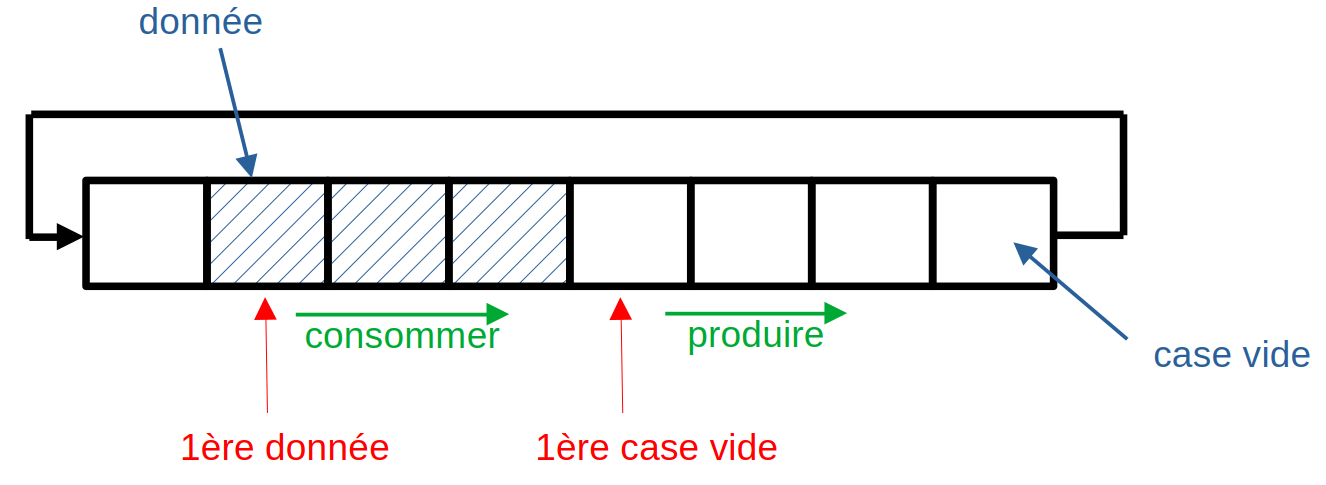
\includegraphics[width=0.7\linewidth]{lecon/18-fil/prod-cons.png}
	\end{center}
	
	\paragraph{Problème :} \begin{itemize}
		\item l'accès au tampon est partagé
		\item les consommateurs doivent attendre qu'une place soir produite
		\item les producteurs doivent attendre que de la place soit libérée dans le tampon.
	\end{itemize}
	
	\paragraph{Solution :} On utilise un sémaphore indiquant le nombre données disponibles et un le nombre de cases disponibles.
	
	\begin{lstlisting}[style=CStyle]
		sem_t mutex, vide, plein;
		sem_init(&mutex, 0, 1);
		sem_init(&vide, 0, N);
		sem_init(&plein, 0, 0);\end{lstlisting}
	
	\begin{minipage}{0.45\textwidth}
		Producteur :
		\begin{lstlisting}[style=Cstyle]
			int item;
			while(1){
				item = produire_item()
				// On attend un place
				sem_wait(&vide);
				sem_wait(&mutex);
				insert_item(item);
				sem_post(&mutex);
				// On la remplie
				sem_post(&plein);
		}\end{lstlisting}
	\end{minipage}\qquad
	\begin{minipage}{0.45\textwidth}
		Consommateur :
		\begin{lstlisting}[style=Cstyle]
			int item;
			while(1){
				// On attend un element
				sem_wait(&plein);
				sem_wait(&mutex);
				item = remove_item();
				sem_post(&mutex);
				// On libere une place
				sem_post(&vide);
				consomer_item(item);
		}\end{lstlisting}
	\end{minipage}
	
\end{appl}

\begin{com}
	Par manque de place, on peut moins s'étendre et ne pas écrire l'algorithme, se contenter de dire qu'on a un sémaphore qui compte les places vides et un les places pleines. (et éventuellement virer le dessin)
\end{com}

\begin{rem}
	On peut implémenter un sémaphore par de l'attente active et des verrous. Donc naturellement, ce qu'apporte souvent les sémaphores, par rapport au verrou, c'est moins d'attente active.
\end{rem}

\begin{com}
	Cette remarque, car si on a des élèves un peu rapide, il pourrait trouver assez facilement des solutions n'utilisant que des verrous, et donc se poserait la question de la pertinence des sémaphores dans ce contexte. L'intérêt des sémaphores vient alors de la suppression de l'attente active.
\end{com}

\section{Interblocage}

\begin{definition}
	On dit qu'il y a interblocage quand tous les fils sont bloqués et ne seront jamais libérés.
\end{definition}

\begin{example} \enspace\\ \normalfont
	\begin{minipage}{0.3\linewidth}
		Fil 1 :
		\begin{lstlisting}[style=CStyle]
			prendre(m1);
			prendre(m2);\end{lstlisting}
	\end{minipage} \quad
	\begin{minipage}{0.3\linewidth}
		Fil 2:
		\begin{lstlisting}[style=CStyle]
			prendre(m2);
			prendre(m1);\end{lstlisting}
	\end{minipage}
\end{example}

\begin{definition}[Diner des philosophes]
	On a cinq philosophes autour d'une table ronde et une fourchette entre chaque. Chaque philosophe alterne moment de faim et de réflexion. Quand il a faim, il attend de prendre ses deux fourchettes, puis il mange, les repose etc.
\end{definition}

\paragraph{Solution naïve :} Un verrou par fourchette, chaque philosopge attend de prendre sa fourchette gauche, puis sa droite

\paragraph{Problème :} Interblocage

\begin{exercise}
	L'implémenter pour observer cet interblocage
\end{exercise}

\paragraph{Solution :} \begin{itemize}
	\item Avec des verrous : chaque philosophe essaye d'abord de prendre sa fourchette de plus petit indice
	\item Avec des sémaphores : On n'autorise que 4 philosophes à essayer de prendre des fourchettes grâce à un sémaphore
\end{itemize}

\begin{com}
	Bon on pourrait aussi mettre dans cette partie un petit dessin.
\end{com}